\documentclass{../../slides-style}

\slidetitle{Особенности синтаксиса Java}{10.10.2026}

\begin{document}

    \begin{frame}[plain]
        \titlepage
    \end{frame}

    \section{Генерики и стирание типов}

    \begin{frame}{Генерики в Java}
        \begin{outline}
            \1 Были добавлены только в Java 5, когда стало понятно, что хранить Object-ы и делать ручной каст --- вообще не дело
                \2 Требовалось обеспечить обратную совместимость, поэтому формат байт-кода было решено не менять
                    \3 Стирание типов
            \1 Генерики в Java инвариантны, массивы ковариантны
        \end{outline}
    \end{frame}

    \begin{frame}{Небольшое отступление про вариантность}
        Ковариантность:
        \begin{center}
            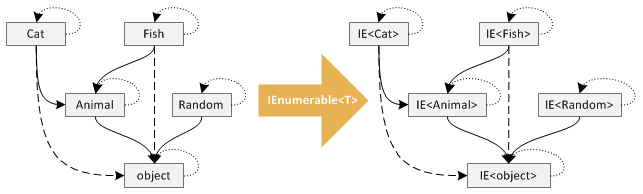
\includegraphics[width=0.6\textwidth]{covariantFunctors.png}
        \end{center}

        Контравариантность:
        \begin{center}
            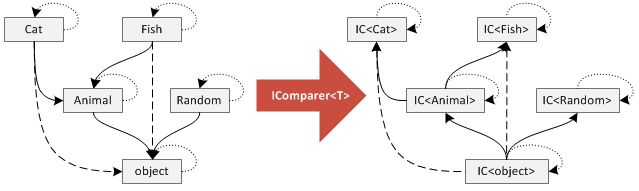
\includegraphics[width=0.6\textwidth]{contravariantFunctors.png}
        \end{center}
        
        \url{http://tomasp.net/blog/variance-explained.aspx/}
    \end{frame}

    \begin{frame}[fragile]{Почему это вообще важно}
        \begin{small}
            \begin{minted}{java}
import org.apache.commons.lang3.tuple.MutablePair;

public void f(MutablePair<Object, Object> x)
{
    ...
}

f(new MutablePair<Object, Object>(apple1, apple2));
f(new MutablePair<Apple, Apple>(apple1, apple2));  // Ошибка компиляции
        \end{minted}
        \vspace{3mm}
        Чтобы нельзя было делать так:
        \begin{minted}{java}
public void f(MutablePair<Object, Object> x)
{
    x.SetLeft(new Battleship());
}
            \end{minted}
        \end{small}
    \end{frame}

    \begin{frame}[fragile]{Массивы ковариантны?}
        \begin{small}
            \begin{minted}{java}
String[] strings = new String[]{"ololo"};
// Всё ок, массив строк является массивом объектов, ковариантность
Object[] objectArray = strings; 
objectArray[0] = 42;  // ArrayStoreException в рантайме
        \end{minted}
        Иначе пришлось бы делать так:

        \begin{minted}{java}
void printNames(Animal[] animals) { ... }
...
Dog[] dogs = new Dog[] {new Dog(), new Dog()};

Animal[] animals = new Animal[dogs.length];
for (int i = 0; i < dogs.length; i++) {
    animals[i] = dogs[i];
}

printNames(animals);
            \end{minted}
        \end{small}
        В C\# то же самое, но это не \enquote{фича}, а legacy языкового дизайна.
    \end{frame}

    \begin{frame}{Wildcards}
        \begin{outline}
            \1 \mintinline{java}|? extends T| --- какой-то подтип T
                \2 Можно читать как T, нельзя записывать ничего, кроме null
                \2 Ковариантность
            \1 \mintinline{java}|? super T| --- надтип T (запись)
                \2 Можно записывать T и его подтипы, читать только как Object
                \2 Контравариантность
            \1 Правило PECS: Producer Extends, Consumer Super
            \1 Ограничения на параметры-типы: \mintinline{java}|<T extends Comparable<T>>| --- T обязан реализовать интерфейс
            \1 В методах, обрабатывающих коллекции, почти всегда нужен wildcard, а не конкретный тип
        \end{outline}
    \end{frame}

    \begin{frame}{Стирание типов}
        \begin{outline}
            \1 Генерики существуют только на этапе компиляции
                \2 Компилятор проверяет и \enquote{стирает} параметры
                    \3 Есть ограничение --- параметр-тип заменяется на верхнюю границу, нет --- на Object
            \1 Поэтому нельзя:
                \2 Создать массив генерик-типа: \mintinline{java}|new T[]| не компилируется
                \2 Перегрузить метод, различающийся только параметром-типом
                \2 Вызвать \mintinline{java}|instanceof List<String>| --- только \mintinline{java}|instanceof List<?>|
                \2 Создать статическое поле типа параметра-типа
                    \3 Статическое поле одно на класс, а для всех инстанциаций генериков класс один
            \1 Приведение к параметру-типу может привести к \mintinline{java}|ClassCastException| в рантайме
            \1 Чем хорошо: не нужен каст при передаче в метод, принимающий сырую коллекцию (старый код)
        \end{outline}
    \end{frame}

    \begin{frame}{Прочие особенности генериков}
        \begin{outline}
            \1 Bridge-методы --- обеспечивают корректный вызов переопределённых в потомке методов
            \1 Обобщённые методы: \mintinline{java}|<T> T max(List<T> list)|
                \2 Параметр выводится из аргументов при вызове
            \1 Типы-обёртки: \mintinline{java}|int| в генерике автоматически становится \mintinline{java}|Integer|
                \2 Строго говоря, генерики value-типов невозможны
        \end{outline}
    \end{frame}

    \begin{frame}[fragile]{Bridge-метод, пример}
        \begin{minted}{java}
class Base<T> {
    public void doWork(T t) { ... } // Стирается до Object
}

class Derived extends Base<String> {
    @Override // Вообще другой метод после стирания
    public void doWork(String s) { ... } 
}
        \end{minted}

        \vspace{1cm}
        Bridge-метод (генерируется компилятором в Derived):

        \begin{minted}{java}
public void doWork(Object t) {
    doWork((String) t);
}
        \end{minted}
    \end{frame}

    \section{Перечисления}

    \begin{frame}{Enum как класс}
        \begin{outline}
            \1 Перечисление --- не список констант, а полноценный тип
            \1 Компилятор создаёт класс, наследующий \mintinline{java}|java.lang.Enum<E>|
            \1 Автоматически генерируются методы
                \2 \mintinline{java}|values()| --- массив всех констант
                \2 \mintinline{java}|valueOf(String)| --- константа по имени
            \1 Константы --- статические поля этого класса
                \2 Технически это значения самого класса (паттерн \enquote{Singleton})
                \2 enum в Java ссылочные!
            \1 В отличие от констант через \mintinline{java}|static final|:
                \2 Типобезопасность (нельзя передать int вместо цвета)
                \2 Возможность добавлять поля и методы
                \2 Можно использовать в switch и в генериках
        \end{outline}
    \end{frame}

    \begin{frame}{Поля, методы и конструкторы в enum}
        \begin{outline}
            \1 В enum можно объявлять поля и методы --- обычные и статические
            \1 Конструктор enum всегда private
                \2 Явный \mintinline{java}|private| --- ошибка компиляции
                \2 Неявный --- конструктор package-private, но вызвать всё равно можно только из тела enum
            \1 Конструктор вызывается при инициализации констант, поэтому константы объявляются первыми
            \1 Данные в константах --- основной способ использования
                \2 Каждая константа несёт свои данные --- технически она объект класса
        \end{outline}
    \end{frame}

    \begin{frame}[fragile]{Enum, пример}
        \begin{small}
            \begin{minted}{java}
public enum Color {
    RED(255, 0, 0),
    GREEN(0, 255, 0),
    BLUE(0, 0, 255);

    private final int r, g, b;

    Color(int r, int g, int b) {
        this.r = r;
        this.g = g;
        this.b = b;
    }

    public String hex() {
        return String.format("#%02x%02x%02x", r, g, b);
    }
}
            \end{minted}
        \end{small}
    \end{frame}

    \begin{frame}[fragile]{У элементов enum тоже могут быть методы!}
        \begin{small}
            \begin{minted}{java}
public enum Operation {
    PLUS {
        @Override
        public double apply(double x, double y) { return x + y; }
    },
    MINUS {
        @Override
        public double apply(double x, double y) { return x - y; }
    };

    public abstract double apply(double x, double y);
}
            \end{minted}
        \end{small}
        \begin{outline}
            \1 Тут enum раскроется компилятором в иерархию классов
            \1 Бесплатная реализация паттерна \enquote{Стратегия}
        \end{outline}
    \end{frame}

    \begin{frame}{EnumSet и EnumMap}
        \begin{outline}
            \1 \mintinline{java}|EnumSet<E>| --- множество на базе битовой маски констант
            \1 \mintinline{java}|EnumMap<K, V>| --- отображение с массивом вместо хеш-таблицы
            \1 Преимущества над HashSet/HashMap:
                \2 Быстрее: доступ по индексу вместо хеширования
                \2 Экономнее память: нет объектов-ключей и служебных структур
            \1 Безопаснее: принимают только нужный enum, не любые объекты
            \1 Почти всегда предпочтительнее, если ключ/элемент --- enum
            \1 \mintinline{java}|EnumSet.noneOf(Color.class)|, \mintinline{java}|EnumSet.of(Color.RED, Color.GREEN)|
        \end{outline}
    \end{frame}

    \begin{frame}{Особенности работы с enum}
        \begin{outline}
            \1 Сравнение --- через \mintinline{java}|==|, не \mintinline{java}|equals|
                \2 Константы --- синглтоны, \mintinline{java}|==| безопасен
                \2 \mintinline{java}|equals| тоже работает, но не нужен
            \1 Нельзя менять порядок объявления констант, если код использует \mintinline{java}|ordinal()|
                \2 И незачем его использовать --- он для реализации ENumSet/EnumMap и прочей внутренней машинерии
            \1 В switch-выражениях компилятор проверяет, что все варианты enum-а покрыты, в старых switch --- нет
        \end{outline}
    \end{frame}

    \begin{frame}{Почему enum-ы в Java такие}
        \begin{outline}
            \1 Типобезопасность: enum-у нельзя присвоить произвольный int даже с кастом, это физически разные типы
            \1 Enum --- полноценное средство моделирования предметной области:
                \2 Связанные данные хранятся прямо в константах
                \2 Можно определять поведение, специфичное для enum, прямо в enum (инкапсуляция)
                \2 Можно определять поведение, специфичное для каждой константы, и использовать полиморфизм
                    \3 В других языках enum часто используется как антипаттерн \enquote{Тэг типа}
            \1 Получился побочный эффект, что enum даже с одним элементом полезен --- бесплатная реализация паттерна \enquote{Одиночка} с безопасным многопоточным доступом
            \1 Близкий аналог --- размеченные объединения в функциональных языках
        \end{outline}
    \end{frame}

    \section{Вложенные классы}

    \begin{frame}{Вложенные классы}
        \begin{outline}
            \1 Static nested class --- объявлен static внутри внешнего класса
                \2 Не имеет доступа к \mintinline{java}|this| внешнего объекта
                \2 Ведёт себя как обычный вложенный класс в других языках
            \1 Inner class --- без static
                \2 Неявно хранит ссылку на внешний объект (Outer.this)
                \2 Для создания нужен экземпляр внешнего класса
                \2 Inner class суть часть целого (отношение композиции)
            \1 Почему Inner class-ы так сделаны:
                \2 Для listener-ов внутри GUI-компонентов, чтобы они могли менять состояние компонента при наступлении события
                    \3 Особенно это полезно для анонимных inner class-ов, которые долгое время играли роль лямбд в Java --- OuterClass.this играл роль \enquote{замыкания для бедных}
                \2 Для поддержки итераторов --- итератор имеет доступ к состоянию коллекции
        \end{outline}
    \end{frame}

    \begin{frame}{Анонимные классы}
        \begin{outline}
            \1 Безымянный класс, наследующий/реализующий тип
            \1 Синтаксис: \mintinline{java}|new Interface() { ... }| или \mintinline{java}|new Superclass(args) { ... }|
            \1 Можно объявлять собственные поля и методы, но они не видны снаружи
                \2 Раз имени у класса нет, кастать не к чему
            \1 Экземпляр создаётся в точке объявления
            \1 Использовались как простой аналог лямбд
        \end{outline}
    \end{frame}

    \begin{frame}[fragile]{Анонимные классы, пример}
        \begin{small}
            \begin{minted}{java}
Runnable r = new Thread() {
    @Override
    public void run() {
        System.out.println("Привет, мир!");
    }
};

Comparator<String> c = new Comparator<String>() {
    @Override
    public int compare(String s1, String s2) {
        return s1.length() - s2.length();
    }
};
            \end{minted}
        \end{small}
    \end{frame}

    \begin{frame}{Захват переменных}
        \begin{outline}
            \1 Анонимный класс может обращаться к переменным метода
            \1 Но только если переменная effectively final --- не изменяется после инициализации
                \2 Компилятор копирует значение в поле класса-замыкания
            \1 Изменить переменную метода из анонимного класса нельзя, поле объемлющего класса --- можно
                \2 Анонимный класс --- честный Inner class, так что имеет OuterClass.this
        \end{outline}
    \end{frame}

    \begin{frame}{Локальные классы}
        \begin{outline}
            \1 Объявляются внутри метода, видны только в нём
            \1 Сочетают свойства анонимных классов и именованных классов
                \2 Есть имя, можно создать несколько экземпляров
                \2 Реализуют интерфейс или расширяют класс
            \1 Могут обращаться к переменным метода, но только если они effectively final
        \end{outline}
    \end{frame}

    \begin{frame}{Доступ к private-членам}
        \begin{outline}
            \1 Вложенные и локальные классы могут обращаться к private-полям и методам внешнего класса
                \2 Технически private-поля они читать не могут, компилятор генерирует Bridge-методы
                    \3 На уровне байт-кода обращаться к private-членам нельзя, JVM не даст, поэтому некий костыль
            \1 Концептуально вложенный класс --- часть реализации внешнего
            \1 Анонимные и локальные классы, объявленные в \emph{статических} методах, OuterClass.this, естественно, не имеют
        \end{outline}
    \end{frame}

    \begin{frame}{Подводные камни}
        \begin{outline}
            \1 Потенциальное нарушение инкапсуляции, поведение размазывается по разным классам
            \1 Вложенный класс держит ссылку на объемлющий, не давая сборщику мусора его собрать
                \2 Пока доступен хоть один итератор, список не удалится --- потенциальная утечка памяти
                \2 Особенно опасно, если это listener, который подписался на какое-то событие из библиотеки, и держит свой this объемлющего класса до конца программы
            \1 Неочевидные зависимости по данным между классами
                \2 У объемлющего класса нет возможности гарантировать, что в его состояние не полезут внутренние классы
            \1 Всё, что можно вынести на верхний уровень без потери смысла --- лучше вынести: меньше связности и удобнее тестировать
        \end{outline}
    \end{frame}

    \section{Лямбды и функциональные интерфейсы}

    \begin{frame}{Функциональные интерфейсы}
        \begin{outline}
            \1 Функциональный интерфейс --- интерфейс ровно с одним абстрактным методом
            \1 \mintinline{java}|@FunctionalInterface| --- проверка компилятором
                \2 Гарантирует, что интерфейс не \enquote{сломается} при добавлении метода
            \1 Стандартные функциональные интерфейсы (\mintinline{java}|java.util.function|):
                \2 \mintinline{java}|Function<T, R>| --- функция
                \2 \mintinline{java}|Predicate<T>| --- предикат, возвращает boolean
                \2 \mintinline{java}|Supplier<T>| --- поставщик, \mintinline{java}|Consumer<T>| --- потребитель
                \2 \mintinline{java}|BiFunction|, \mintinline{java}|UnaryOperator| и др.
            \1 Можно писать свои
        \end{outline}
    \end{frame}

    \begin{frame}{Лямбды}
        \begin{outline}
            \1 Анонимные функции для реализации функциональных интерфейсов
                \2 По сути, синтаксический сахар для анонимных классов
                    \3 Но реализации несколько отличаются, лямбда может побыстрее работать
            \1 Синтаксис: \mintinline{java}|(параметры) -> тело|
                \2 Например, \mintinline{java}|Runnable r = () -> System.out.println("Hi")| или \mintinline{java}|list.stream().filter(s -> s.length() > 3)|
            \1 Замыкания --- как в анонимных классах, effectively final-переменные и поля объемлющего класса
                \2 Лямбда имеет OuterClass.this и держит на него ссылку
                \2 В C\# захват переменных \enquote{по ссылке}, так что нет ограничения на effectively final, но есть способ прострелить себе ногу
            \1 Лямбда --- объект
        \end{outline}
    \end{frame}

    \begin{frame}{Ссылки на методы}
        \begin{outline}
            \1 Сокращение от лямбды, когда тело --- просто вызов метода: \mintinline{java}|String::length|
            \1 Четыре формы:
                \2 Статический метод: \mintinline{java}|Integer::parseInt|
                \2 Метод экземпляра привязанного объекта: \mintinline{java}|string::length| --- метод запускается от объекта string
                \2 Метод экземпляра непривязанный: \mintinline{java}|String::length| --- метод запускается от объекта, который ему передадут первым аргументом при вызове
                    \3 Например, \mintinline{java}|list.stream().map(String::length)|
                \2 Конструктор: \mintinline{java}|ArrayList::new|
            \1 Ссылки на методы могут быть несколько хуже по читаемости
                \2 Тем более что статические методы принимают аргументы как есть, а нестатические непривязанные принимают первым аргументом this
        \end{outline}
    \end{frame}

    \begin{frame}[fragile]{Ограничения лямбд}
        \begin{outline}
            \1 Нельзя объявить поля и вспомогательные методы --- тело может быть только выражением или блоком (с фигурными скобками)
            \1 Нет собственного \mintinline{java}|this| --- это \mintinline{java}|this| окружающего контекста
                \2 Ну им и не надо, раз у них полей и методов нет
            \1 Нельзя пробрасывать checked-исключения
                \begin{footnotesize}
                    \begin{minted}{java}
Runnable r = () -> { throw new IOException(); }; // не компилируется
                    \end{minted}
                \end{footnotesize}
                \2 Разумно, checked-исключения негде задекларировать
                \2 Обходной путь --- обернуть в unchecked или свой функциональный интерфейс с throws в сигнатуре
            \1 Нельзя создать переменную с именем, занятым параметром лямбды
        \end{outline}
    \end{frame}

    \begin{frame}{Типизация лямбд}
        \begin{outline}
            \1 Целевой тип выводится из контекста
                \2 Ищется функциональный интерфейс, метод которого принимает значения нужных типов и возвращает значение нужного типа
                \2 Если их несколько --- ошибка компиляции
                    \3 Тогда явно указываем тип: \mintinline{java}|f((FuncInt) () -> System.out.println("Hi"));| или \mintinline{java}|FuncInt lambda = () -> System.out.println("Hi");|
            \1 Лямбда не создаёт класс в исходном коде
                \2 В байткоде --- bootstrap‑метод + вызов \mintinline{java}|invokedynamic|
                \2 При первом вызове JVM решает, что делать (сгенерить реальный объект, заинлайнить, ...)
                \2 При последующих вызовах переиспользуется результат первого
            \1 Анонимный класс и лямбда ведут себя по-разному при захвате \mintinline{java}|this|
                \2 Если лямбда ничего не захватывает, this не хранится
                \2 Игра-угадайка для сборки мусора
                    \3 Не полагайтесь на оптимизацию захвата this, следите за памятью
        \end{outline}
    \end{frame}

    \begin{frame}{Анонимный класс или лямбда}
        \begin{outline}
            \1 Лямбда предпочтительнее для одного функционального метода: короче, компактнее
            \1 Анонимный класс лучше, когда:
                \2 Нужно состояние --- собственные поля, изменяемые между вызовами
                \2 Реализуется несколько методов (не функциональный интерфейс)
                \2 Нужна перегрузка конструктора суперкласса с разными аргументами
            \1 Исторически: анонимные классы --- до Java 8, лямбды --- основной способ с Java 8
        \end{outline}
    \end{frame}

    \section{Исключения}

    \begin{frame}{Иерархия исключений}
        \begin{outline}
            \1 \mintinline{java}|Throwable| --- всё, что можно бросить и поймать
                \2 \mintinline{java}|Error| --- фатальные ошибки JVM и ресурсов (OutOfMemoryError, StackOverflowError), обычно не обрабатываем
                \2 \mintinline{java}|Exception| --- предсказуемые, но не ожидаемые ошибки, обрабатываем
            \1 RuntimeException и его наследники --- unchecked
                \2 NullPointerException, IndexOutOfBoundsException, IllegalArgumentException
            \1 Остальные Exception --- checked
                \2 IOException, SQLException, ParseException
            \1 Ошибка программиста --- это unchecked, ошибка среды --- чаще checked
            \1 Если ошибка ожидаема и может возникнуть при нормальной работе программы (например, ошибка пользовательского ввода) --- \emph{исключения не используем}
        \end{outline}
    \end{frame}

    \begin{frame}{Checked и unchecked исключения}
        \begin{outline}
            \1 Checked: компилятор заставляет либо перехватить (\mintinline{java}|catch|), либо объявить \mintinline{java}|throws|
            \1 Аргументы \enquote{за} checked:
                \2 Невозможно пропустить обработку ошибки, контракт виден в сигнатуре и проверяется компилятором
            \1 Аргументы \enquote{против}:
                \2 Размывают контракт: исключение может всплыть из любой глубины
                \2 Побуждают к пустым catch-блокам и бросанию наружу через десятки методов
                \2 Неудобно в функциональном стиле и лямбдах
            \1 Современный тренд (в т.ч. в новых API JDK) --- отдавать предпочтение unchecked
            \1 Checked --- восстановимые ошибки (перечитать файл, повторить запрос)
        \end{outline}
    \end{frame}

    \begin{frame}{Работа с исключениями, хорошие практики}
        \begin{outline}
            \1 Сохранять причину: \mintinline{java}|throw new IllegalStateException(e)|
                \2 Или \mintinline{java}|initCause/getCause|, \mintinline{java}|new Ex(e, message)| в собственных исключениях
            \1 Не терять стек: не делайте \mintinline{java}|throw new ...| в catch
                \2 Тем более без initCause
            \1 Писать собственные исключения, если стандартные слишком общие
            \1 Не использовать исключения для управления потоком выполнения
            \1 Исключение --- не бесплатное, занимает время и память
                \2 Стек в Java может быть очень длинным
        \end{outline}
    \end{frame}

    \section{Современная Java}

    \begin{frame}[fragile]{Expression switch}
        \begin{small}
            \begin{minted}{java}
enum Level { DEBUG, INFO, WARN, ERROR }

int priority = switch (level) {
    case DEBUG -> 1;
    case INFO -> 2;
    case WARN -> {
        System.out.println("Warning level detected");
        yield 3;
    }
    case ERROR -> {
        if (critical) {
            yield 5;
        } else {
            yield 4;
        }
    }
};
            \end{minted}
        \end{small}
    \end{frame}

    \begin{frame}{Pattern matching и выражения}
        \begin{outline}
            \1 Pattern matching для \mintinline{java}|instanceof| (Java 16):
                \2 \mintinline{java}|if (obj instanceof String s)| --- переменная \mintinline{java}|s| уже типизирована
                \2 Похоже на smart cast в Kotlin, но требует нового имени
            \1 Pattern matching для \mintinline{java}|switch| (Java 21):
                \2 \mintinline{java}|switch (obj) { case String s -> ...; case Integer i -> ...; }|
            \1 Текстовые блоки (Java 15): \mintinline{java}|""" ... """| 
                \2 Для SQL, HTML, JSON без \mintinline{java}|\n|
        \end{outline}
    \end{frame}

    \begin{frame}{Record и sealed}
        \begin{outline}
            \1 \mintinline{java}|record| (Java 16) --- класс для хранения данных
                \2 Конструктор, геттеры (\mintinline{java}|x()|, не \mintinline{java}|getX()|), equals/hashCode/toString --- автоматически
                \2 Поля финальные, класс финальный
                \2 Используется для хранения немутабельных данных (Data Transfer Objects)
                \2 Спасает от кучи boilerplate-кода
            \1 \mintinline{java}|sealed| (Java 17) --- контролируемое наследование
                \2 Перечисляет разрешённых наследников: \mintinline{java}|permits Shape, Circle|
                \2 В паре с pattern matching компилятор проверяет полноту switch
                \2 enum-ы как раз sealed
                \2 В Kotlin тоже есть sealed, но там все наследники должны быть в одном файле, в Java они явно перечисляются и могут быть где угодно
        \end{outline}
    \end{frame}

    \begin{frame}[fragile]{Implicitly declared classes}
        \begin{outline}
            \1 JEP 445 и далее (Java 21+ preview, стабилизировано в Java 25)
            \1 Тело \mintinline{java}|main| можно писать без объявления класса и метода:
                \begin{footnotesize}
                    \begin{minted}{java}
// раньше
public class Main {
    public static void main(String[] args) {
        System.out.println("Hello!");
    }
}

// теперь (Java 21+, preview)
System.out.println("Hello!");
                    \end{minted}
                \end{footnotesize}
            \1 Компилятор неявно объявляет класс и main
            \1 Пока дополняет, а не заменяет обычный стиль: библиотечный код, модули и привычная структура остаются прежними
            \1 Языковой дизайн \enquote{Хочу как в Python} --- минимизировать накладные расходы при написании простых программ
                \2 В C\# так же
        \end{outline}
    \end{frame}

    \section{Рефлексия}

    \begin{frame}{Рефлексия вообще}
        \begin{outline}
            \1 Механизм получения compile-time-информации во время выполнения
            \1 В разных языках имеет разные возможности (от очень ограниченной RTTI в C++ до весьма развитой в .NET)
                \2 В интерпретируемых языках (JavaScript, Python) не нужна --- программа и так знает о себе всё
            \1 Нужна много где, от создания плагинных систем в приложениях до сериализации и юнит-тестов
            \1 Реализуется хранением информации о типах в скомпилированной программе
                \2 В нашем случае в байт-коде
                    \3 В Java рефлексия \enquote{уважает} стирание типов --- параметры-типы генериков ей недоступны
            \1 Как правило, язык дополнительно расширяется аннотациями (или атрибутами)
                \2 Произвольная информация, \enquote{надеваемая} на сущности программы, которую можно использовать в рантайме
        \end{outline}
    \end{frame}

    \begin{frame}{Class и получение типов}
        \begin{outline}
            \1 Объект \mintinline{java}|Class<T>| --- описание типа в рантайме
            \1 Три основных способа получить его:
                \2 \mintinline{java}|obj.getClass()| --- у существующего объекта
                \2 \mintinline{java}|T.class| --- по имени типа
                \2 \mintinline{java}|Class.forName("com.example.Foo")| --- по строке, загружает класс
            \1 Через \mintinline{java}|Class| открываются методы, поля, конструкторы, аннотации, generic-суперклассы
            \1 Есть загрузчик класса (ClassLoader), именно он грузит классы из CLASSPATH, его можно использовать вручную
        \end{outline}
    \end{frame}

    \begin{frame}{Доступ к полям и методам}
        \begin{outline}
            \1 Получение членов класса:
                \2 \mintinline{java}|getDeclaredMethods()|, \mintinline{java}|getDeclaredFields()|
                \2 Также \mintinline{java}|getDeclaredConstructors()|; объявленные в классе без учёта наследования
                \2 Для наследуемых --- \mintinline{java}|getMethods()|
            \1 Приватные члены доступны, но надо вызвать \mintinline{java}|setAccessible(true)|, чтобы ими воспользоваться
            \1 Создание объекта: \mintinline{java}|clazz.getDeclaredConstructor().newInstance()|
                \2 Странное \enquote{clazz} используется как имя для переменной с классом, потому что \mintinline{java}|class| --- ключевое слово
            \1 Вызов метода по строке: \mintinline{java}|method.invoke(obj, args)|
        \end{outline}
    \end{frame}

    \begin{frame}{Аннотации и стирание}
        \begin{outline}
            \1 Аннотации доступны рефлексией, только если retention --- \mintinline{java}|RUNTIME|
                \2 \mintinline{java}|SOURCE| --- виден компилятору (Override, SuppressWarnings)
                    \3 Линтеры, кодогенераторы и т.п.
                \2 \mintinline{java}|CLASS| --- остаётся в class-файле, но не виден в рантайме
                    \3 Для инструментов, работающих с байт-кодом (AOT-компилятторы, обфускаторы и т.п.)
                \2 Retention --- аннотация к аннотациям, указывается при объявлении аннотации
            \1 Чтение: \mintinline{java}|clazz.getAnnotation(Deprecated.class)|, аннотации на методах и параметрах
            \1 Стирание проявляется и здесь:
                \2 Нельзя получить тип параметра поля: \mintinline{java}|List<String> field| виден рефлексией только как \mintinline{java}|List|
            \1 Аннотации не влияют на поведение сами по себе
        \end{outline}
    \end{frame}

    \begin{frame}[fragile]{Как использовать}
        \begin{small}
            Объявление аннотации:
            \begin{minted}{java}
@Retention(RetentionPolicy.RUNTIME)
@Target(ElementType.METHOD)
public @interface MyTest { }
            \end{minted}

            \vspace{5mm}
            Использование аннотации:
            \begin{minted}{java}
public class TestRunner {
    public static void runTests(Object instance) throws Exception {
        for (Method m : instance.getClass().getMethods()) {
            if (m.isAnnotationPresent(MyTest.class)) {
                m.invoke(instance);
            }
        }
    }
}
            \end{minted}
        \end{small}
    \end{frame}

    \begin{frame}{Ограничения и цена рефлексии}
        \begin{outline}
            \1 Производительность: вызов через рефлексию заметно медленнее прямого
                \2 \mintinline{java}|MethodHandles| (с Java 7) быстрее, но не так гибко
            \1 Инкапсуляция и модули JPMS:
                \2 С Java 9 доступ к internals других модулей ограничен
                \2 \mintinline{java}|setAccessible(true)| может выбросить \mintinline{java}|InaccessibleObjectException|
            \1 Слабая типобезопасность: ошибки имен классов и методов ловятся в рантайме
            \1 Хрупкость: переименование поля ломает все обращения по строкам
            \1 Безопасность: рефлексия позволяет обходить приватность, поэтому её ограничивают в песочницах и в module-info.java
        \end{outline}
    \end{frame}

    \begin{frame}{Lombok}
        \begin{outline}
            \1 Библиотека, генерирующая код на этапе компиляции
            \1 Основные аннотации:
                \2 \mintinline{java}|@Data| --- геттеры, сеттеры, equals/hashCode/toString, конструктор из полей
                \2 \mintinline{java}|@Getter| / \mintinline{java}|@Setter| --- точечно
                \2 \mintinline{java}|@Value| --- только геттеры, equals/hashCode/toString, конструктор из полей
                    \3 В современной Java есть \mintinline{java}|record|
                \2 \mintinline{java}|@Builder| --- сгенерируется реализация паттерна \enquote{Builder}
                \2 \mintinline{java}|@NoArgsConstructor| / \mintinline{java}|@AllArgsConstructor|
            \1 Спасает от кучи boilerplate-кода, особенно из-за отсутствия property в Java
        \end{outline}
    \end{frame}

    \begin{frame}{Как работает Lombok}
        \begin{outline}
            \1 Annotation Processing (JSR 269): компилятор вызывает обработчик аннотаций и вставляет сгенерированный код в AST
                \2 По сути, это плагин к компилятору, реализующий javax.annotation.processing.Processor
                    \3 Можно (и легко) свой написать
            \1 На выходе обычный class-файл с дополнительными методами
                \2 Ничего не происходит в рантайме
            \1 Отсюда особенности:
                \2 Нужна поддержка IDE (плагин Lombok) --- иначе не видны сгенерированные методы
                \2 Сложнее отлаживать: в исходниках метода нет
                \2 Lombok \enquote{не знает} о ваших методах, написанных руками, и может конфликтовать
                \2 Так что record предпочтительнее
        \end{outline}
    \end{frame}

\end{document}
